\subsection{Proposed Work}

\subsubsection{Class-wise CIEs: Mitigating The Bias problem for Fairness in Edge Inference}
The most black-box way to understand a network is to study the classification it provides for different input classes.  This does not tell us how the network arrives at the classification, but it contains more fine-grained information than the aggregate accuracy.  Figure~\ref{fig:r56Output-class-wise} illustrates 
%\ggcmtside{Move "Impact of ResNete56... from being a title to the caption. Also label the Y axis. Also merge with Figure 4 -- or maybe not!}
how a state-of-the-art compression tool~\cite{joseph2019programmable} affects the error in certain classes more significantly than others --- something we wish to avoid as it may result in unfair treatment~\cite{hooker2019selective}. 

\begin{figure}[!h]
    %\begin{minipage}[t]{0.55\linewidth}
    \centering
    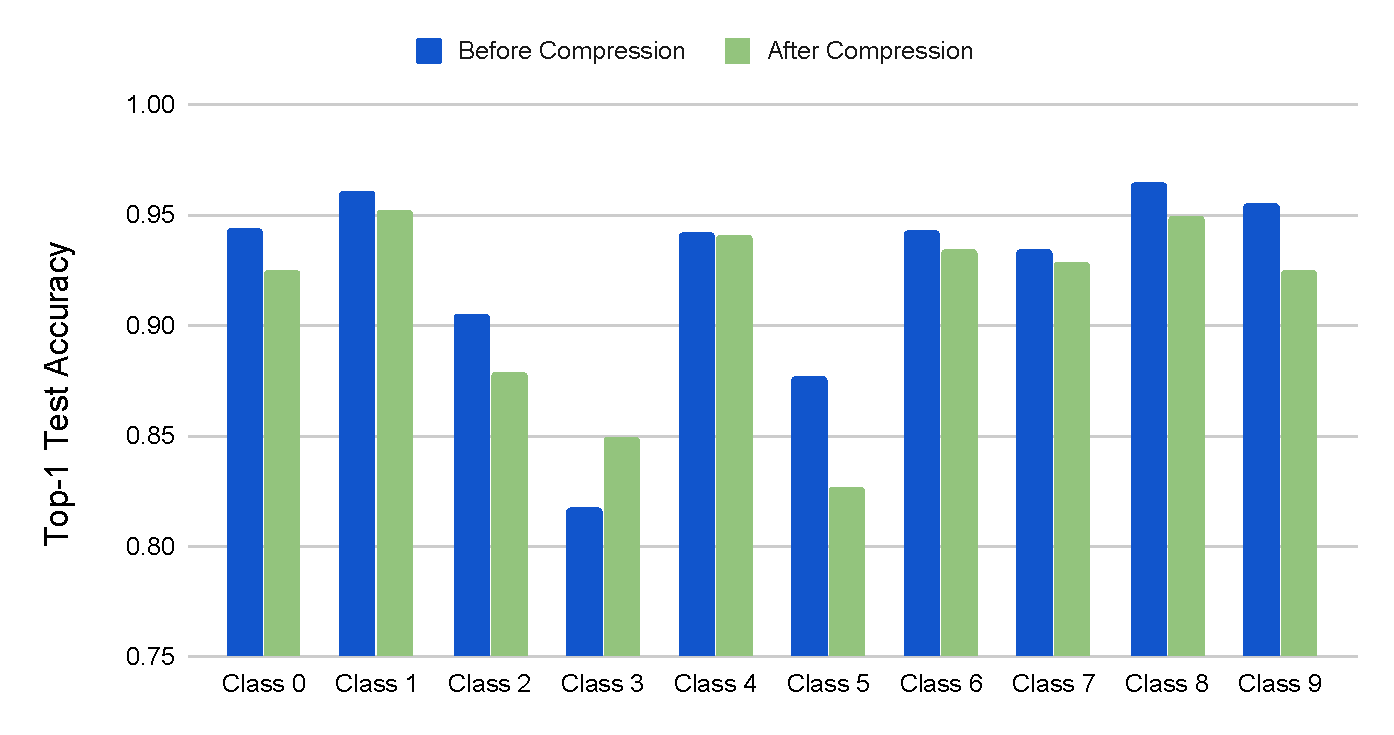
\includegraphics[width=\linewidth,clip,trim=0 .25in 0 0]{img/class-impact.pdf}
    %\vspace{-0.2in}
    \caption{\small Effect of compression on class-wise accuracy (CIFAR-10 with ResNet56 architecture)}
    \label{fig:r56Output-class-wise}
    %\end{minipage}%
\end{figure}

While class-wise accuracy numbers are more nuanced than the overall accuracy, they are still a coarse representation of the underlying issues. For example, we often observe ``structure'' in the misclassifications: some classes are much more likely to be misclassified as a few other classes than the rest of the classes.  That is, compression may result in one mammal being misclassified as another mammal, but very rarely as an object. This distinction can be important for safety and security, and depending on the application (e.g., autonomous driving, home cameras), some misclassifications are more costly than others. We capture this distinction using an application-specific metric or a distance function $d(y_1,y_2)$ between classes $y_1$ and $y_2$ (see~\cite{qin2018verification}). Denoting the reference and the compressed networks by $f$ and $\widetilde{f}$ respectively (these are functions mapping the inputs $\bx$ to labels $y$), the total misclassification cost of $\widetilde{f}$ relative to $f$ is
\[ \Delta_{\mu, d}(\widetilde{f}, f) :=  \sum_{\bx} \mu (\bx) d(\widetilde{f}(\bx), f(\bx)),\]
where $\mu(\bx)$ is the weight of the input $\bx$.  The main questions we study are, \textit{(1)} how do known compression algorithms perform with respect to the above metric for different choices of $d$ and the reference network? \textit{(2)} how can we incorporate this metric into the compression procedure?\label{tmc-measure}
%

Answering the first question will lead to an understanding of which compression scheme is better for a given application. Also, it may suggest that some reference networks are more compressible than others while maintaining semantic information. Such trends have been observed in our current framework \condensa{}~\cite{joseph2019programmable}. 
%\ggcmtside{Is this where to refer to this figure? It was not referenced before. I also made up the caption. Check it.} 
%
Answers to the second question will lead us to
better domain-specific compression. 
%
Given a metric $d$ and weights $\mu$, the \ardent{} system will allow a user to optimize the standard training loss, while incorporating constraints on $\Delta_{\mu, d}$.  To achieve this, we need a notion of the derivative of the distance $d$, which provides a direction for changing $\widetilde{f}$ that reduces the objective. One natural way to define this is to make $\widetilde{f}(\bx)$ move towards $f(\bx)$.  But depending on the structure of the metric $d$, better definitions are possible. To illustrate, if an image $\bx$ of a husky is misclassified as a chair, it may suffice (for certain applications) to move $\widetilde{f}(\bx)$ towards one of the dog classes, and not necessarily a husky. This weaker requirement could lead to better compression.  \ardent{} will allow ways to specify $d$ that allow such optimization, including hierarchical metrics (cf.~\cite{Babenko2009SimilarityMF,Bengio2010Label}) and metrics 
where the class labels are embedded in a Euclidean space.\label{hier-metrics}

\subsubsection{Attribution Matching for Sensitive Edge Inference Tasks}

\paragraph{Motivation}
Mitigating the impact of compression is particularly
urgent given the widespread use of compressed deep 
neural networks in resource constrained but sensitive 
domains such as 
%
%
%
health care diagnostics 
\cite{xie2019automated, %(Xie et al., 2019; 
gruetzemacher20183d,    %Gruetzemacher et al., 2018; 
badgeley2019deep,       %$Badgeley et al., 2019;
oakden2020hidden}       %Oakden-Rayner et al., 2019),
%
%
,self-driving cars 
\cite{teslacrash17} %(NHTSA, 2017)
%
facial recognition software
\cite{
buolamwini2018gender% Buolamwini
 % Gebru, 2018b). 
} and
%
hiring
\cite{amazon18, 
yourface19}.% Harwell2019
%
%
For these tasks, the trade-offs incurred by 
compression will be intolerable given the huge impact 
on human welfare.
%
Due to the success of Deep learning, there is an 
emergent trend to utilize deep neural networks (DNNs) 
even for safety-critical applications such as 
self-driving cars and health-care applications 
\cite{estava2017dermatologist,
samala2018evolutionary, lane2018deep}.
%
Due to the inherent nature of such devices, 
it is of paramount importance that the utilized 
DNNs be reliable and trustworthy to human users.
%

For a system to be reliable, perpetual service 
must be rendered and the integrity of the system 
must hold even under unexpected circumstances.
%
%
For most commercially deployed DNNs, this condition 
is hardly met as they are often operated in the 
cloud due to their heavy computational requirements.
%
%
However, this dependence on clouds acts as a 
critical weakness in safety-sensitive settings 
as intermittent communication failuers to the 
cloud may cause difficulties in reacting to 
situations immediately, or even-worse, 
the device's connection to the cloud may be 
severed indefinitely.
%
%
Thus, to guarantee reliable service, 
the DNNs must be embedded on the edge device.
%
%
%
To this end, network compression techniques such 
as pruning \cite{han2015deep,li2016pruning} and distillation \cite{hinton2015distilling,zagoruyko2016paying} 
are commonly employed - as a compressed network 
would require less computational time and memory 
but maintain its prediction performance to a 
certain acceptable margin, effectively substituting 
the original network for edge computation.

At the same time, for a system to be trustworthy, 
the system must be transparent enough for humans 
to understand its workings and the reasons for its outputs.
%
%
An example would be when a health monitor 
predicts an onset of disease \cite{xu2019current}
- then the clinician would require an acceptable
explanation to the device output.
%
%
However, the black-box nature of deep neural 
networks complicates this goal - impeding its 
advance in safety-critical areas.
%
%
For DNNs to gain trustworthiness, the ability 
to explain why the network makes such decisions 
is essential. Such field of interest - 
eXplainable AI (XAI) - has emerged as one of the 
importance frontiers in the field of deep learning.
%
%
Amoung numerous XAI methods, the most commonly 
used methods are attribution methods \cite{selvaraju2017grad}, 
which weigh the parts of the input data according to 
how much they 'contributed' to produce the output prediction.
%
%
Such attribution methods are beginning to be applied
in safety-critical fields \cite{liang2020prediction}.

To ensure the safety of the system, 
the two aforementioned conditions should be simultaneously 
satisfied - the embedded DNNs must be equipped with 
both compression and attribution.
%
%
However we show for the first time that these seemingly
unrelated techniques conflict with each other:
compressing a network causes deformations in 
the produced attributions, even if the predictions 
of the network stays the same before and after compression.
%
%
\vcmt{This is a potentially severe crack in the 
integrity of the compressed network, 
as the premise in which a compressed network 
is acceptable in safety-critical fields is that 
the compressed network in as reliable as its former self}.
%
%
\textit{This implies that the compressed nework must behave 
almost identically to the pre-compression network while being
smaller in size.}
%
%
Moreover, the classifications between the network are
not only different from their past counterparts 
but also broken down compared to their respective ground truths
%
%
\begin{itemize}
    \item Examples where the compressed model gets the example 
          right but the uncompressed model gets it wrong.
    \item Examples where the uncompressed model gets it right 
          but the compressed model gets it wrong.
\end{itemize}
%
%
These label distortions directly
cause incorrect interpretations, which could lead to dire 
consequences for safety-critical systems.
%
%
Such a problem arises from the pitfall of existing 
network compression approaches: they only
aim to maintain the prediction quality of the network while 
reducing the size of the network.
%
%
Compressing a network forces the network to cram its 
necessary decision procedures and information inside a
smaller space.
%
This space restriction forces the network to abandon its 
standard decision procedures and resort to using shortcuts 
and hints that are seemingly indecipherable to humans.
%
Thus, its decision procedures would become harder to 
interpret, which is reflected in its production of deformed
attribution maps
%
%
To resolve this newfound unintended
issue, we propose a novel label-preservation aware 
compression framework  to ensure both the reliability and 
trustworthiness of the compressed model.
%
...we concentrate on the observation that the labels 
of the pre-network (teacher) are closer to the ground truth signal 
compared to the post-network (student).
%
Thus, in the absence of ground truth signals, the labels
of the teacher can serve as a proxy. 
%
In this sense, we propose a automatically parameter 
tuned regularizer learning framework that matches the 
of the now-compressing network to its attribution maps 
before compression, transferring the attributional power 
of the pre-network to the post-network. Our work sheds 
new light on transfer learning techniques from the perspective of XAI,
as they can be re-interpreted and subsumed under our framework.

In many safety-critical
applications,
  one may have constraints  
  such as
  ``{\sl the two networks focus on the same aspects of an image},'' or 
  ``{\sl certain aspects of an image are not used for classification}.''  To incorporate such constraints, we propose the using methods from interpretability research such as saliency maps and influence attribution~\cite{SimonyanVZ13,fergus2013Visualizing,Kim2018Interpretability,Mukund2017Axiomatic}.
  %\ggcmtside{Give a one-sentence definition of influence attribution?} 
  These techniques give a way to ``trace'' the factors in an input that contributed to the overall classification.  Given a network and an input image $\bx$, a method such as~\cite{Mukund2017Axiomatic,Kim2018Interpretability} outputs the influence (or attribution score) of each pixel on the overall classification.

 
\begin{figure}[!htb]
    \centering
    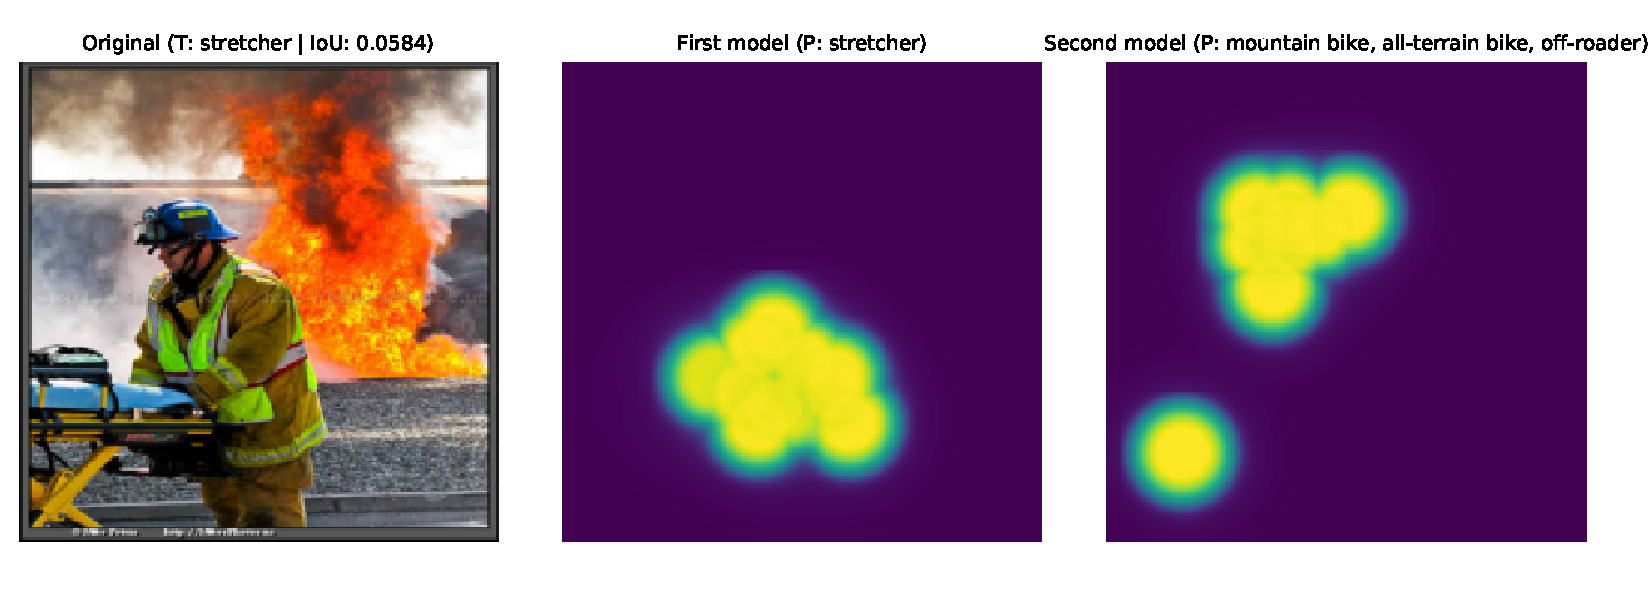
\includegraphics[width=\linewidth]{img/fire.pdf}
    %\vspace{-0.2in}
    \caption{\small Image from ImageNet's \textit{stretcher} class, along with saliency maps showing the parts of the image ``most responsible'' for classification by the reference and compressed models. Former obtains the correct class, while the latter classifies as {\em mountain bike, all-terrain bike}.}
    \label{fig:fire}
    %\vspace{-0.2in}
\end{figure}

Interestingly, we find that in many cases of discrepancy between the reference and the compressed model (e.g., Figure~\ref{fig:fire}), the attributions differ significantly, indicating that the two models focus on different regions of the input.  Given the attribution scores $\alpha$ and $\alpha'$, we consider the weighted Jaccard similarity (a generalization of the natural {\em intersection-over-union} (IoU)) metric:%\ggcmtside{Cite IoU, ensure reviewer feels included.}
\[ \text{sim}(\alpha, \alpha') = \frac{ \sum_i \min( \alpha_i, \alpha'_i )}{\sum_i \max (\alpha_i, \alpha'_i) }. \]
When deploying a compressed network, a natural goal is to have high value for this similarity.  This can help avoid possible security issues during deployment (as we will discuss in Section~\ref{mu-tech}),
 and in general lead to a higher agreement between the models.
\label{fse-metric}
%One reason is that the reference network may have been carefully trained to avoid specific biases (e.g. skin color), and we do not want the compression procedure to introduce bias. Another (informal) reason is that a high similarity score implies that both networks are using the {\em same features} of an image, which makes them more likely to agree on the classification.
\ardent{} will support incorporating the $\text{sim}()$ objective during compression, and moreover, this will be done for a range of attribution methods (including but not limited to~\cite{SimonyanVZ13,Mukund2017Axiomatic,ancona2018towards}).